%%%%%%%%%%%%%%%%%%%%%%%%%%%%%%%%%%%%%%%%%
% Jacobs Landscape Poster
% LaTeX Template
% Version 1.1 (14/06/14)
%
% Created by:
% Computational Physics and Biophysics Group, Jacobs University
% https://teamwork.jacobs-university.de:8443/confluence/display/CoPandBiG/LaTeX+Poster
% 
% Further modified by:
% Nathaniel Johnston (nathaniel@njohnston.ca)
%
% This template has been downloaded from:
% http://www.LaTeXTemplates.com
%
% License:
% CC BY-NC-SA 3.0 (http://creativecommons.org/licenses/by-nc-sa/3.0/)
%
%%%%%%%%%%%%%%%%%%%%%%%%%%%%%%%%%%%%%%%%%

%----------------------------------------------------------------------------------------
%	PACKAGES AND OTHER DOCUMENT CONFIGURATIONS
%----------------------------------------------------------------------------------------

\documentclass[final]{beamer}

\usepackage[scale=1.24]{beamerposter} % Use the beamerposter package for laying out the poster

\usetheme{confposter} % Use the confposter theme supplied with this template

\setbeamercolor{block title}{fg=ngreen,bg=white} % Colors of the block titles
\setbeamercolor{block body}{fg=black,bg=white} % Colors of the body of blocks
\setbeamercolor{block alerted title}{fg=white,bg=dblue!70} % Colors of the highlighted block titles
\setbeamercolor{block alerted body}{fg=black,bg=dblue!10} % Colors of the body of highlighted blocks
% Many more colors are available for use in beamerthemeconfposter.sty

%-----------------------------------------------------------
% Define the column widths and overall poster size
% To set effective sepwid, onecolwid and twocolwid values, first choose how many columns you want and how much separation you want between columns
% In this template, the separation width chosen is 0.024 of the paper width and a 4-column layout
% onecolwid should therefore be (1-(# of columns+1)*sepwid)/# of columns e.g. (1-(4+1)*0.024)/4 = 0.22
% Set twocolwid to be (2*onecolwid)+sepwid = 0.464
% Set threecolwid to be (3*onecolwid)+2*sepwid = 0.708

\newlength{\sepwid}
\newlength{\onecolwid}
\newlength{\twocolwid}
\newlength{\threecolwid}
% \setlength{\paperwidth}{48in} % A0 width: 46.8in
% \setlength{\paperheight}{36in} % A0 height: 33.1in
\setlength{\sepwid}{0.024\paperwidth} % Separation width (white space) between columns
\setlength{\onecolwid}{0.22\paperwidth} % Width of one column
\setlength{\twocolwid}{0.464\paperwidth} % Width of two columns
\setlength{\threecolwid}{0.708\paperwidth} % Width of three columns
\setlength{\topmargin}{-0.5in} % Reduce the top margin size
%-----------------------------------------------------------

\usepackage{graphicx}  % Required for including images

\usepackage{booktabs} % Top and bottom rules for tables

%----------------------------------------------------------------------------------------
%	TITLE SECTION 
%----------------------------------------------------------------------------------------

\title{EpiMed Platform: Concept-driven analysis of omics data in translational research context} % Poster title

\author{Sophie Rousseaux, Anne-Laure Vitte, Florent Chuffart, Ekaterina Flin} % Author(s)

\institute{IAB (U1209/UMR5309)} % Institution(s)

%----------------------------------------------------------------------------------------

\begin{document}

\addtobeamertemplate{block end}{}{\vspace*{2ex}} % White space under blocks
\addtobeamertemplate{block alerted end}{}{\vspace*{2ex}} % White space under highlighted (alert) blocks

\setlength{\belowcaptionskip}{2ex} % White space under figures
\setlength\belowdisplayshortskip{2ex} % White space under equations

\begin{frame}[t] % The whole poster is enclosed in one beamer frame

\begin{columns}[t] % The whole poster consists of three major columns, the second of which is split into two columns twice - the [t] option aligns each column's content to the top

\begin{column}{\sepwid}\end{column} % Empty spacer column

\begin{column}{\twocolwid} % The first column

%----------------------------------------------------------------------------------------
%	OBJECTIVES
%----------------------------------------------------------------------------------------

\begin{alertblock}{Objectives}

EpiMed: Medical Epigenetics and Bioinformatics

\begin{itemize}
\item Facilitate a translational research in epigenetics, between the fundamental research teams and the medical teams.
\item Analyze large-scale whole-genome data that is essential to understand the epigenome.
\item Organize an interactive database associating “omics” data with biological and clinical data.
\end{itemize}

\end{alertblock}


%----------------------------------------------------------------------------------------
%	INTRODUCTION
%----------------------------------------------------------------------------------------

\begin{block}{Concept driven omics analysis}

The main research activity of EpiMed is discovery of new biomarkers in cancers based on ectopic expression of tissue-specific genes \cite{rousseaux:hal-01261754}.

{
\centering
\mbox{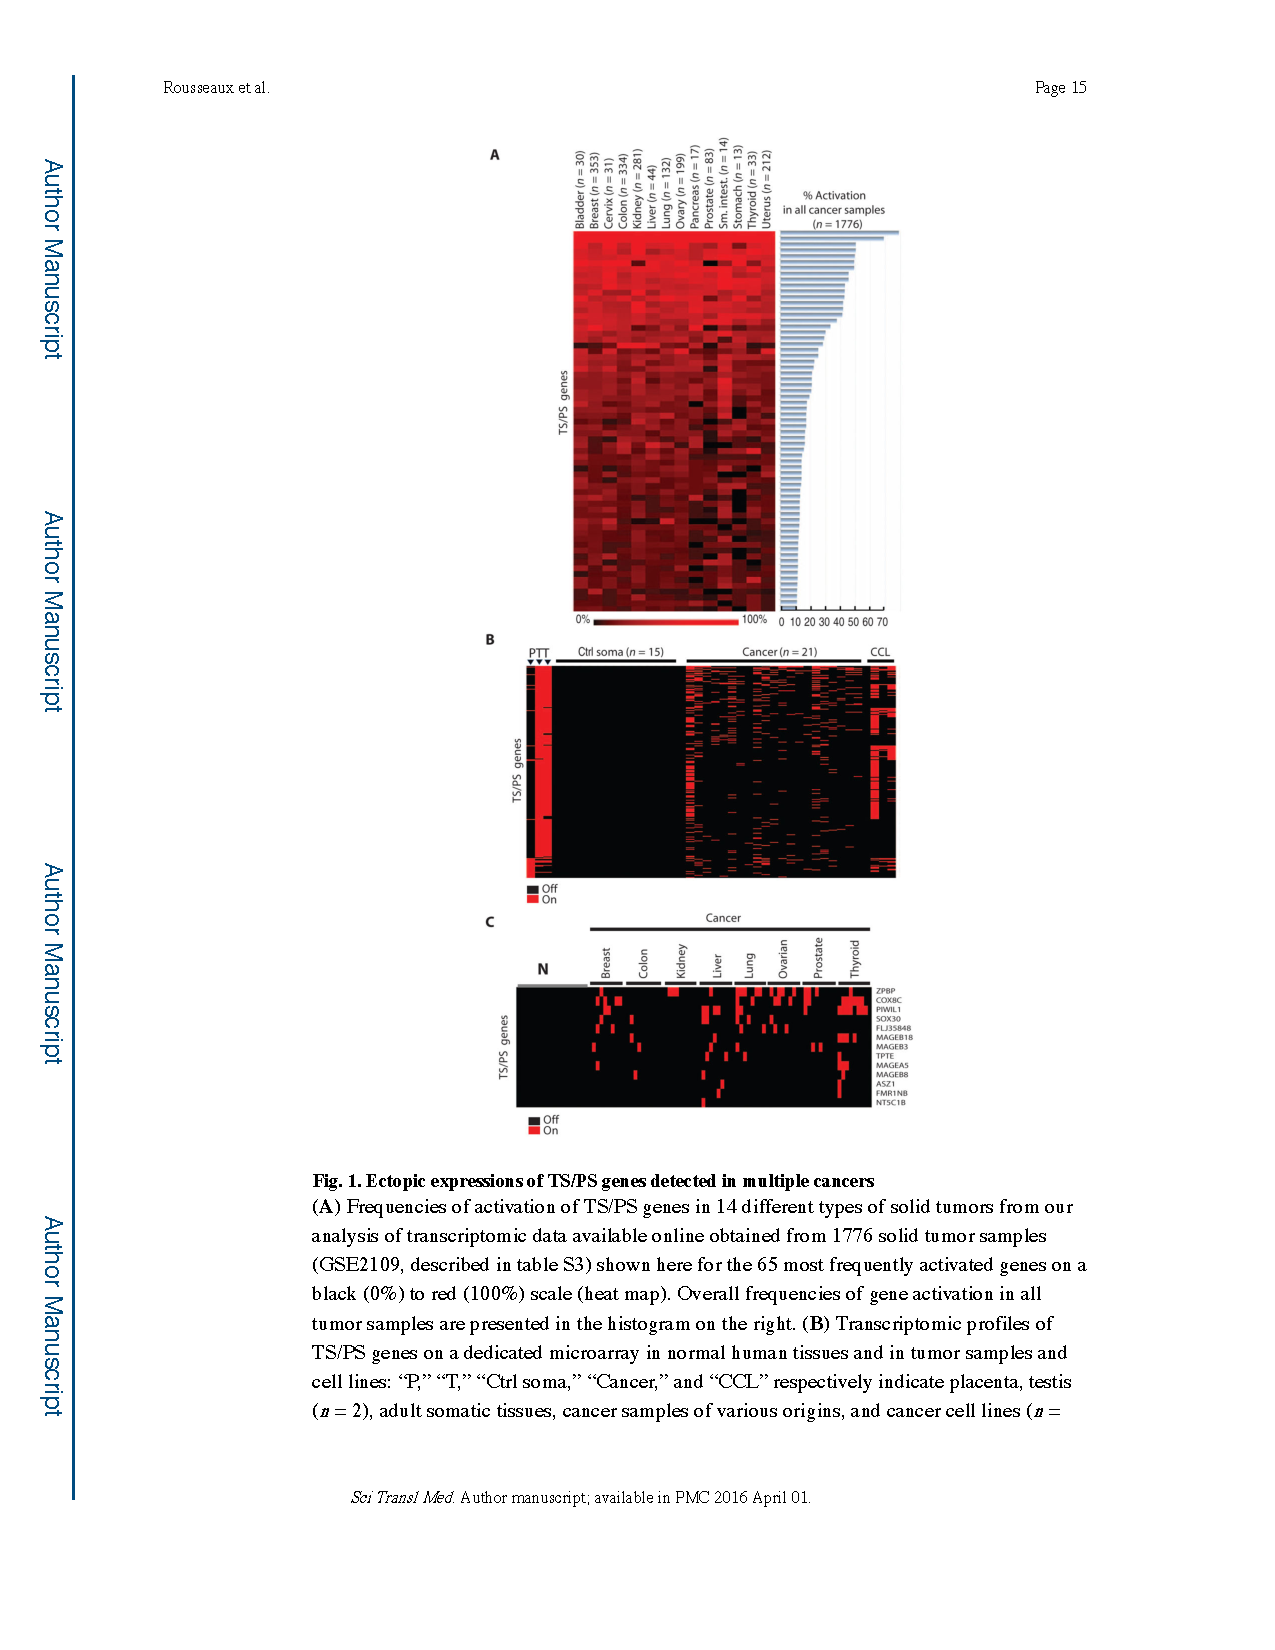
\includegraphics[trim = 85mm 125mm 60mm 107mm, clip, width=.58\linewidth]{figs/fig01}}
\mbox{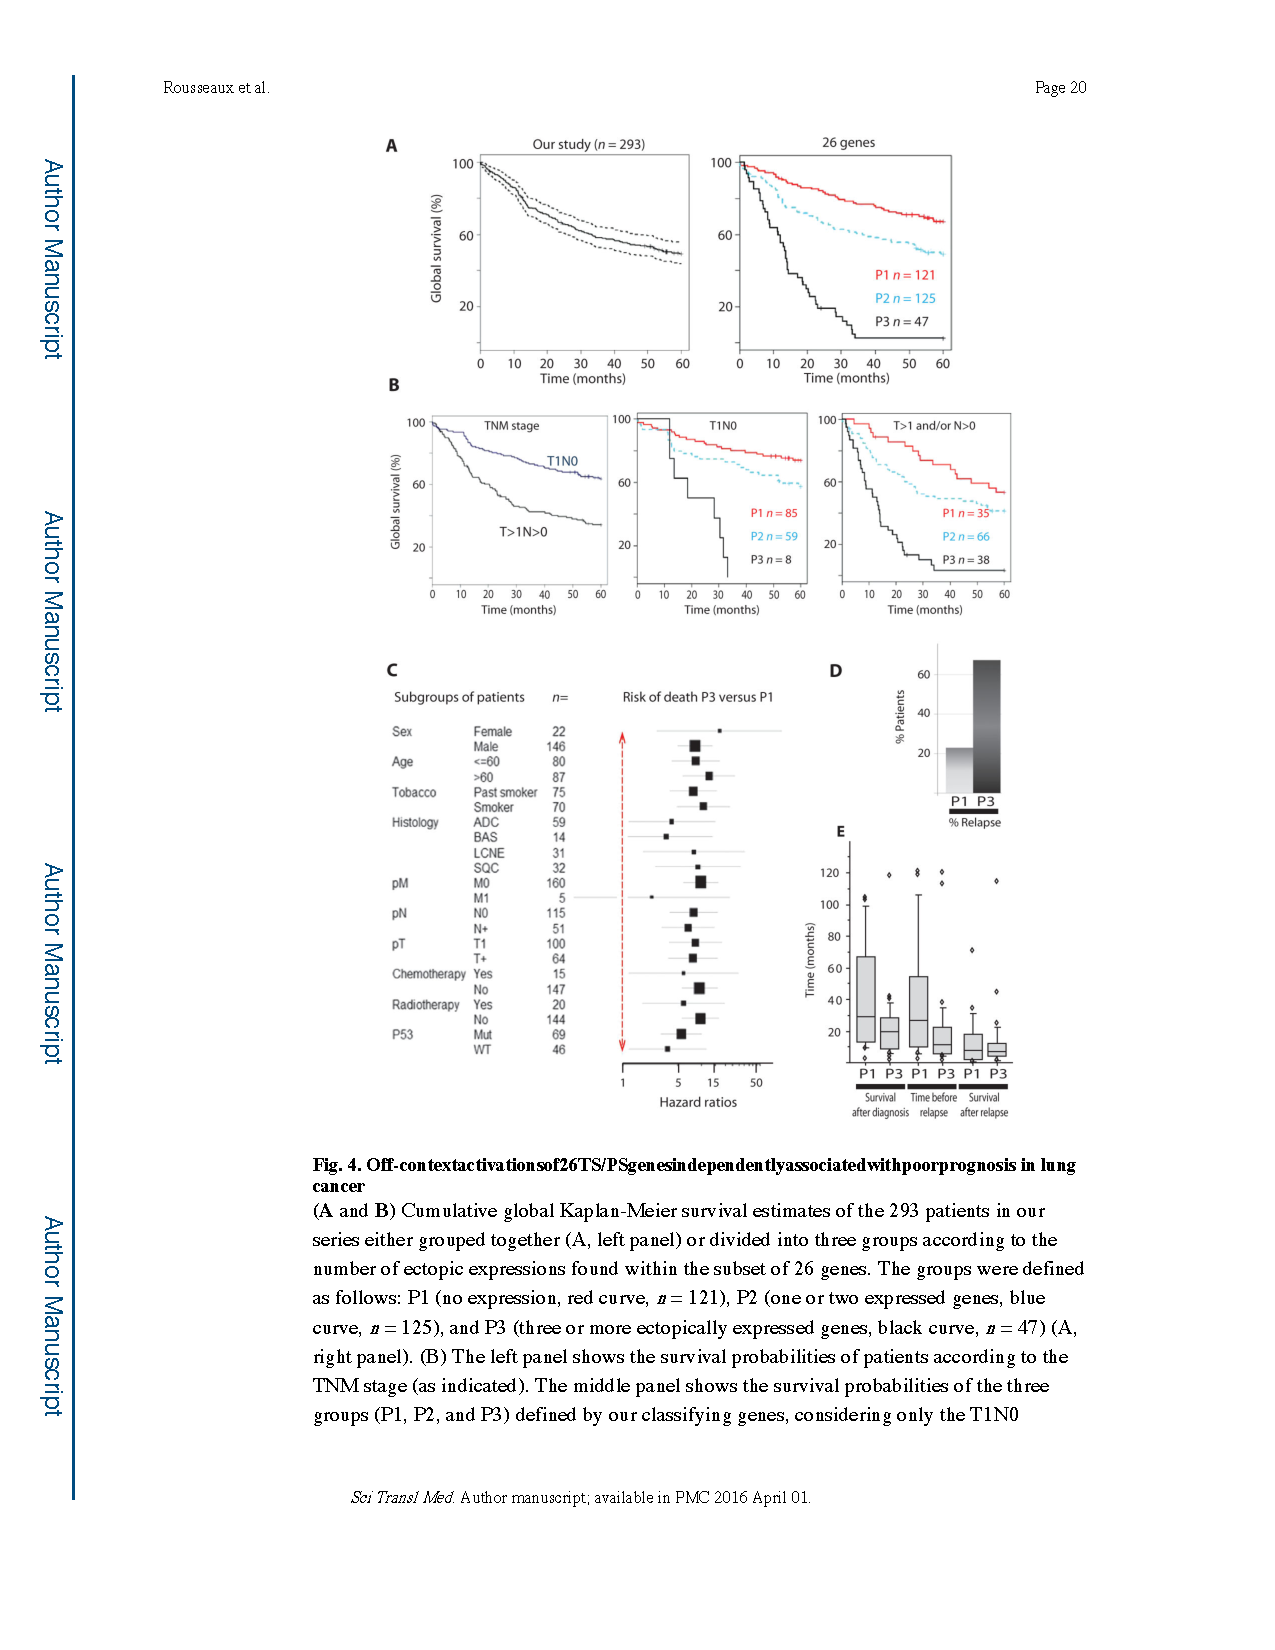
\includegraphics[trim = 120mm 212mm 50mm 20mm, clip, width=.4\linewidth]{figs/fig02}}
}

% [Rousseaux et al., Sci Transl Med, 2013.]

% II. Scientific collaborations

We develop specific pipelines of data processing dedicated to each research project. Data analysis is driven by scientific questions and concepts.

% Collaborative network:
% \begin{itemize}
% \item IAB, CHU, TIMC-IMAG, GIN, LJK,
% \item International collaborations
% \end{itemize}


III. Expertise, Services and Tools 

\begin{itemize}
\item Expertise in bioinformatics, biostatistics, HPC, machine learning
\item EpiMed Database for clinical data and omics meta-data queries
\item R package “epimedtools” for omics data processing and analysis
\end{itemize}

\end{block}
%----------------------------------------------------------------------------------------


















\begin{block}{EpiMed Database and Interfaces}

EpiMed Database provide tools for “omics” meta-data management

{
\centering
\mbox{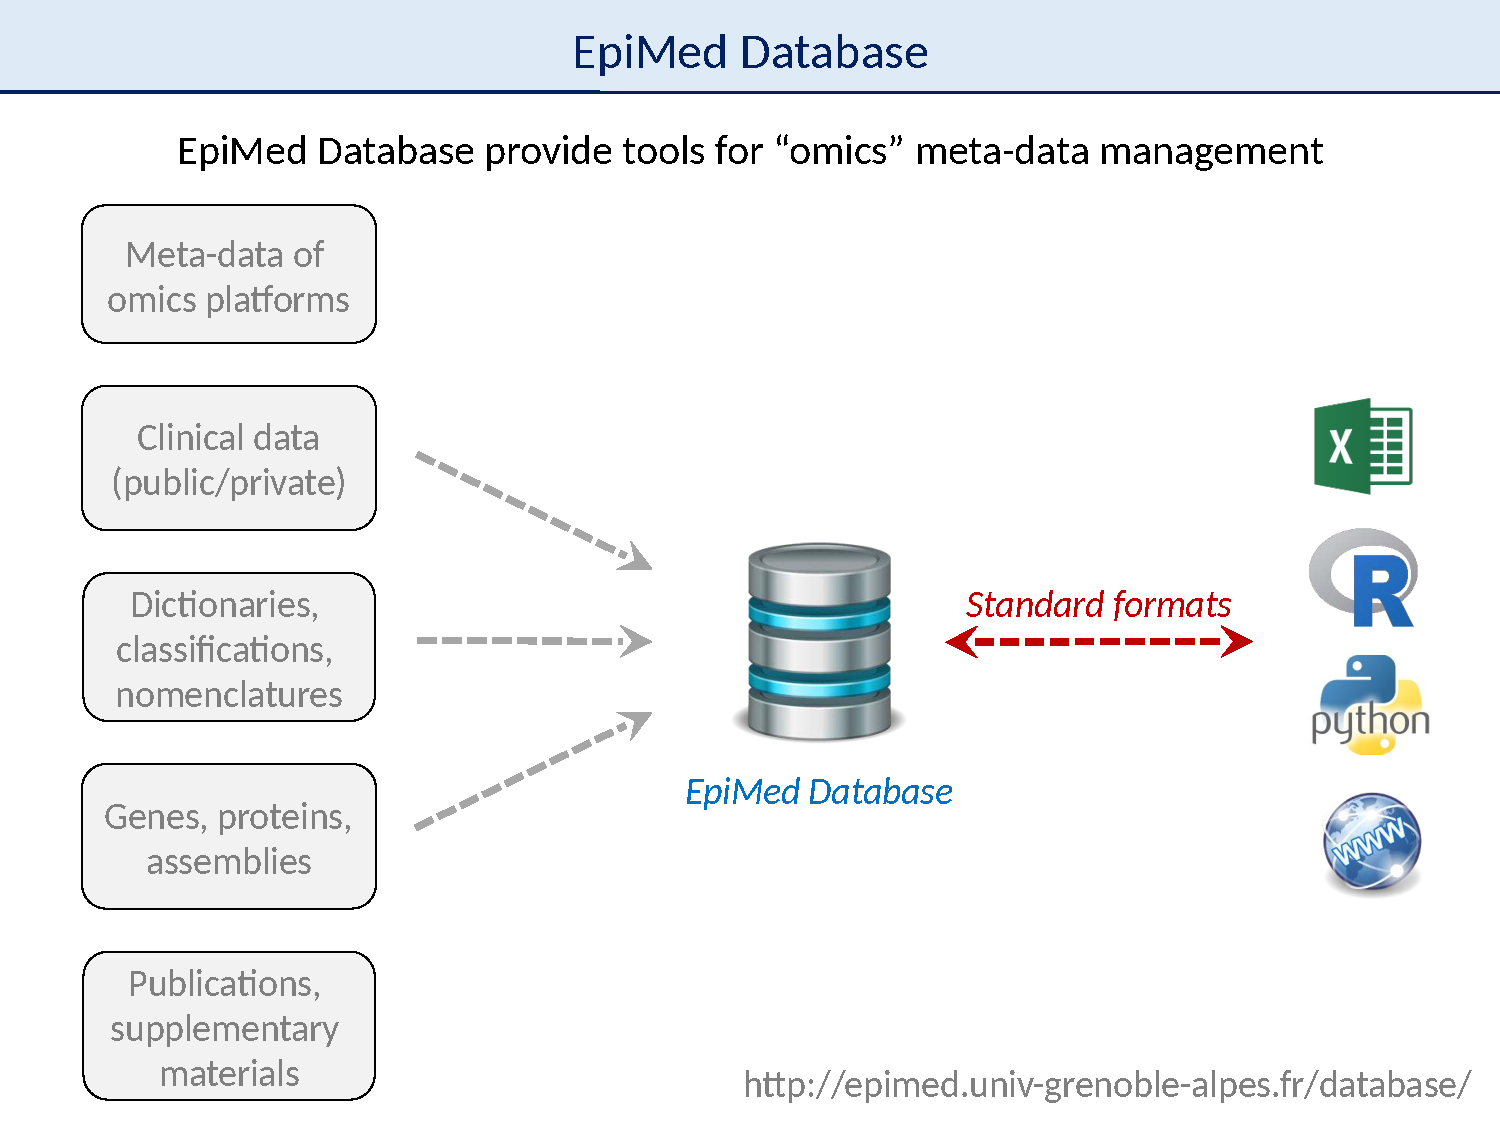
\includegraphics[trim = 0mm 0mm 0mm 30mm, clip, width=.6\linewidth]{figs/fig03}}

}

Tools are reachables using web interfaces and more...

{
\centering
\mbox{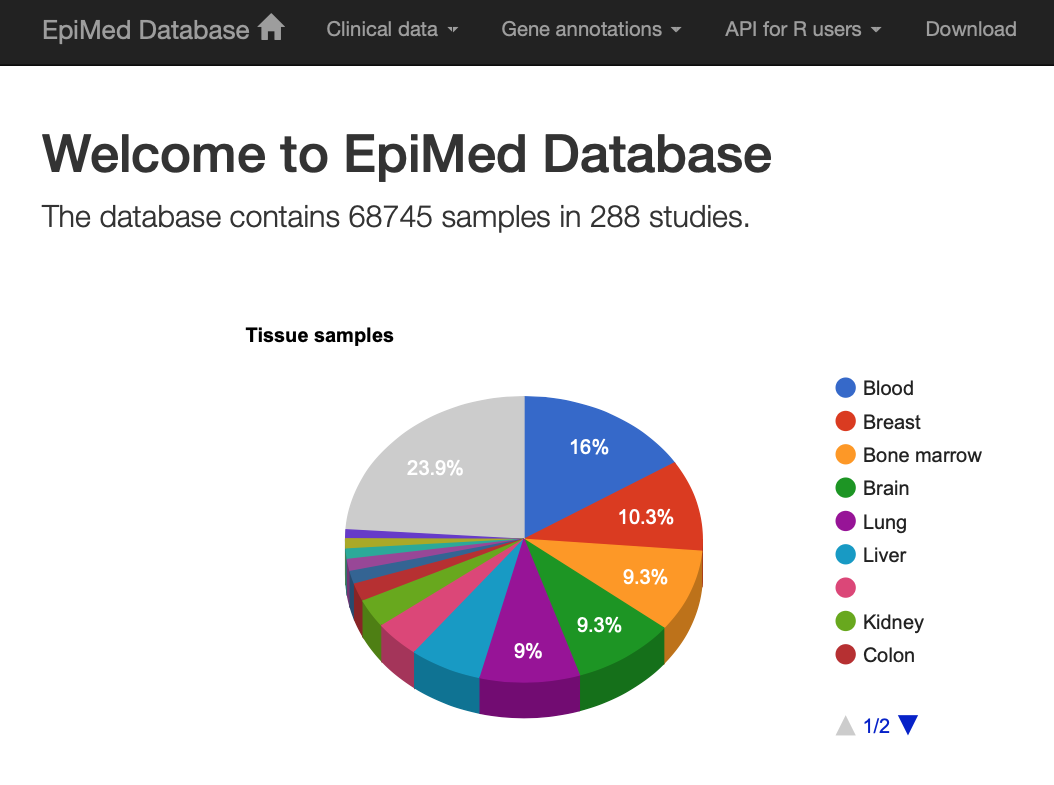
\includegraphics[trim = 0mm 0mm 0mm 00mm, clip, width=.6\linewidth]{figs/fig03b}}

}

\end{block}






\end{column} 





























\begin{column}{\sepwid}\end{column} % Empty spacer column

\begin{column}{\twocolwid} % The third column












\begin{block}{EpiMed Expertise}


EpiMed platform knits different kinds of collaborations
and deals with heterogenous data

{
\centering
\mbox{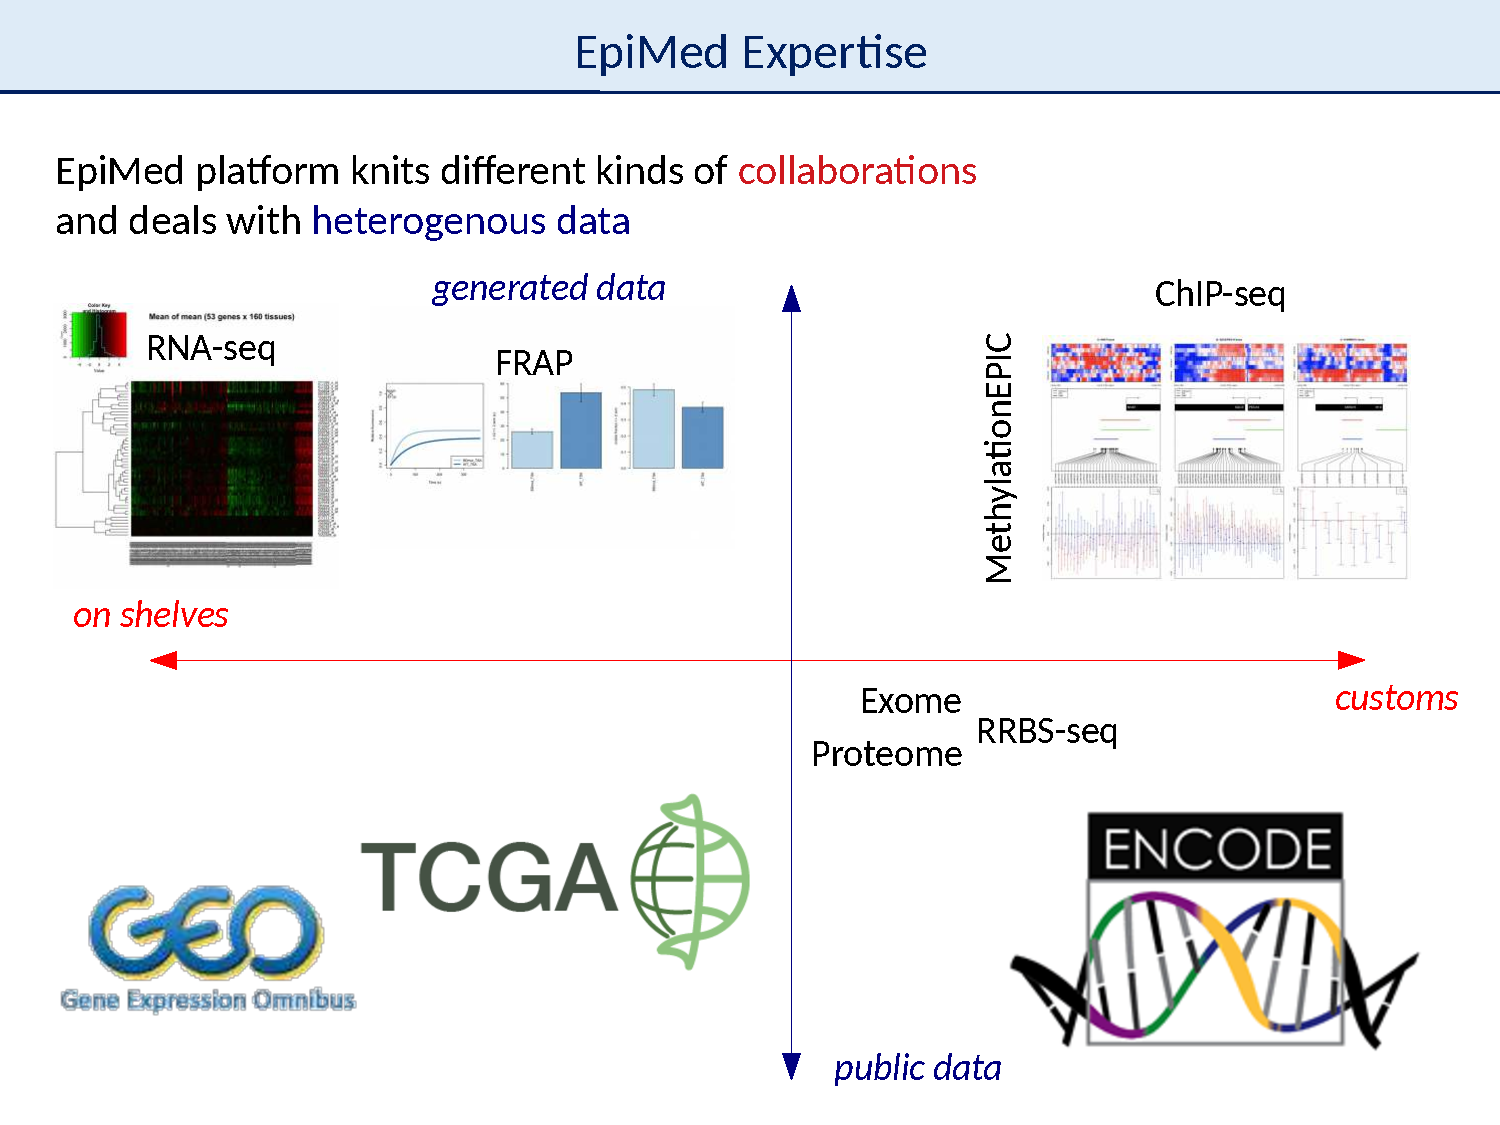
\includegraphics[trim = 0mm 0mm 0mm 43mm, clip, width=.9\linewidth]{figs/fig04}}

}

\end{block}







\begin{block}{Example of RNA-seq analysis on cell lines}
{
\centering
\mbox{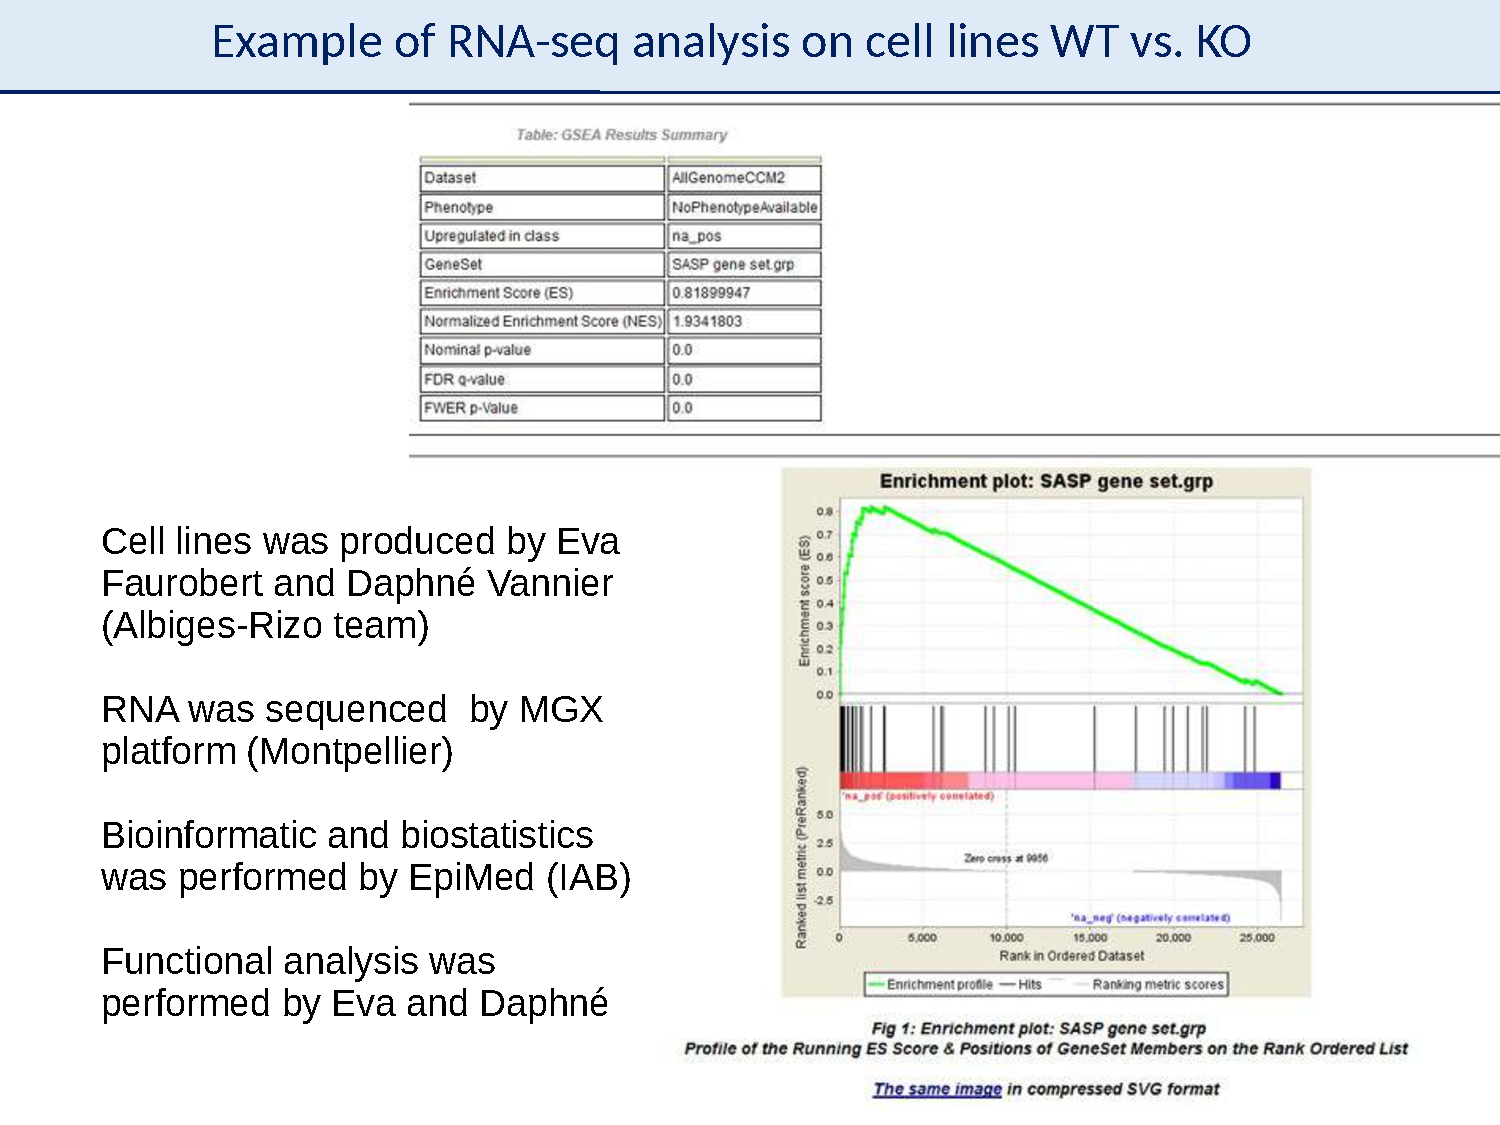
\includegraphics[trim = 0mm 0mm 0mm 43mm, clip, width=.66\linewidth]{figs/fig05}}

}
\end{block}











\begin{block}{Proteomics-Transcriptomics interface}

Beijing – Shanghai - Grenoble, Lung Cancer Total Proteomic: 100 cancer + 100 non-tumoral

{
\centering
\mbox{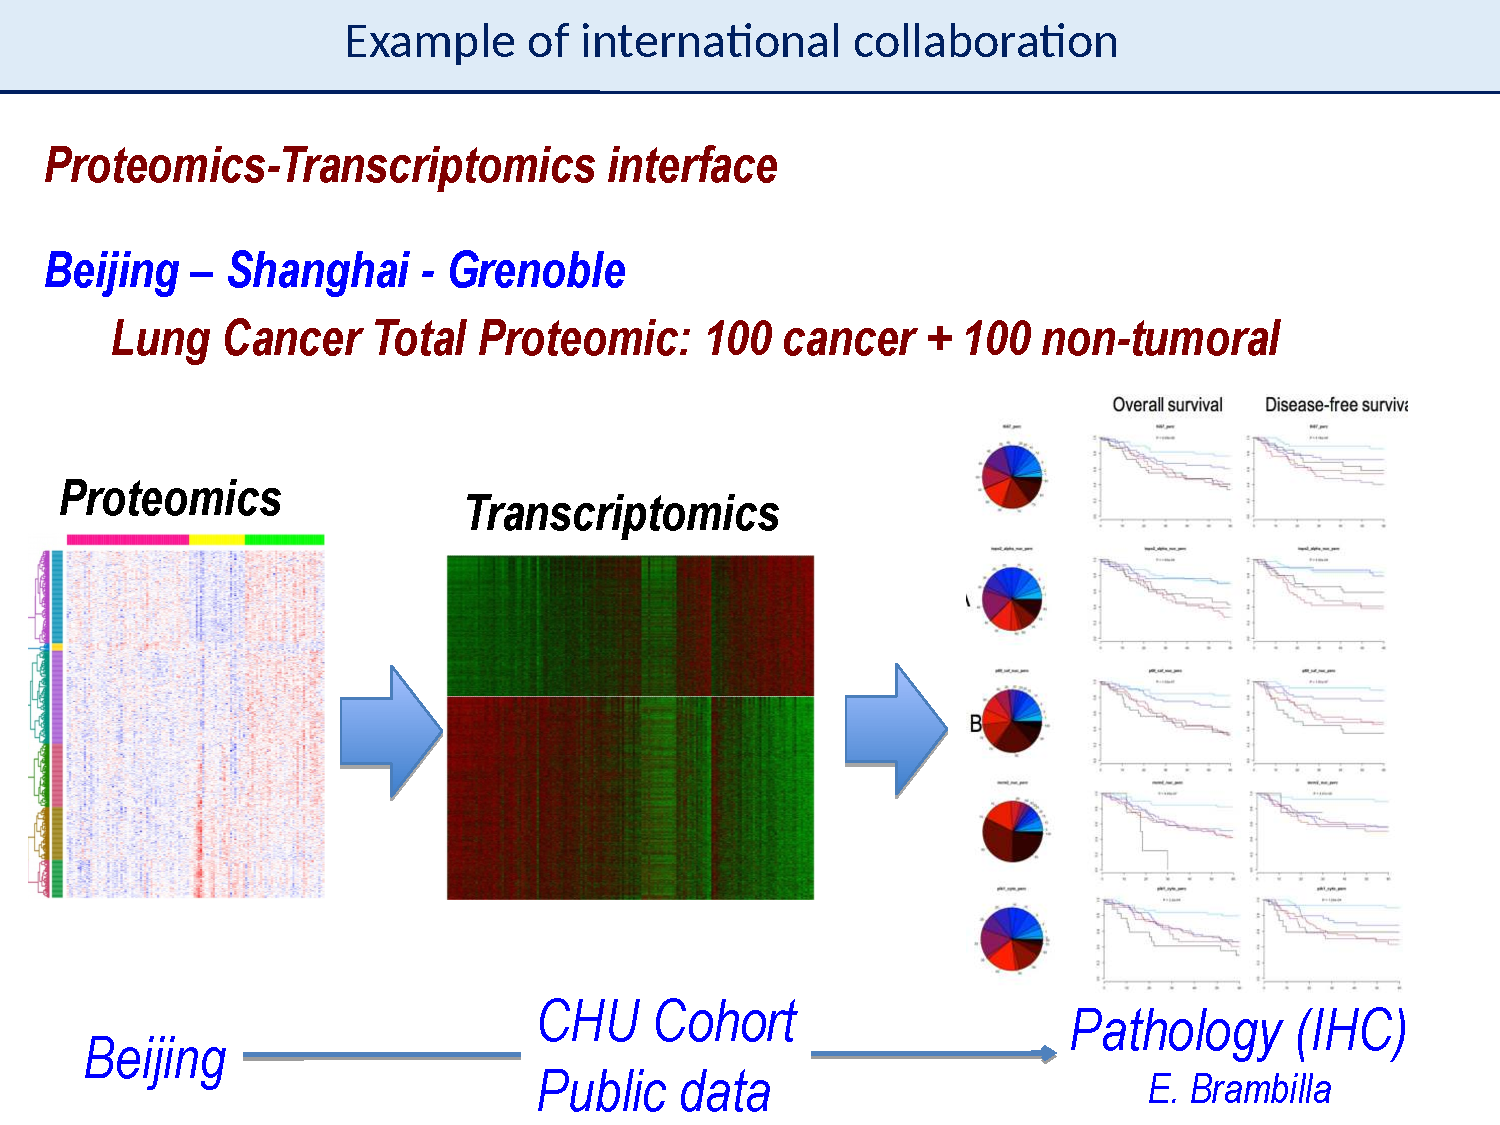
\includegraphics[trim = 0mm 0mm 0mm 63mm, clip, width=.66\linewidth]{figs/fig06}}

}
\end{block}





\begin{block}{Eden cohort}
{

Collaboration with Johanna Lepeule

\centering
\mbox{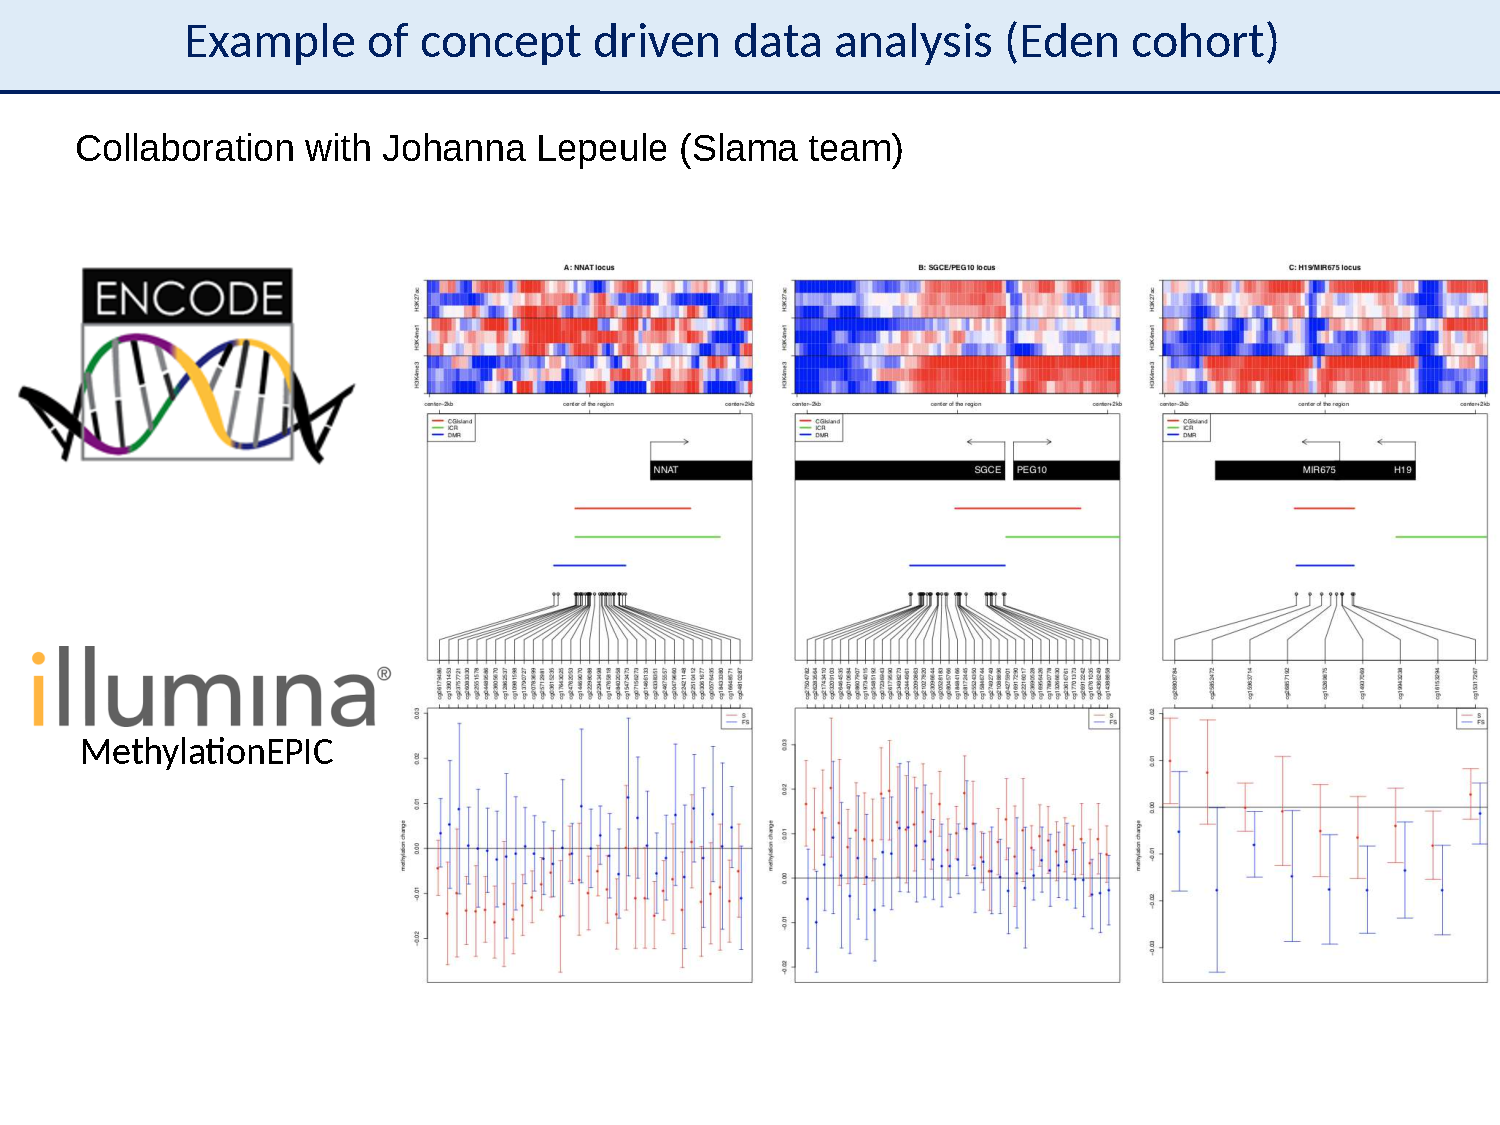
\includegraphics[trim = 0mm 0mm 0mm 43mm, clip, width=.66\linewidth]{figs/fig07}}

}
\end{block}





% %----------------------------------------------------------------------------------------
% %  REFERENCES
% %----------------------------------------------------------------------------------------
%
% \begin{block}{References}
%
% \nocite{*} % Insert publications even if they are not cited in the poster
% \small{\bibliographystyle{unsrt}
% \bibliography{biblio}\vspace{0.75in}}
%
% \end{block}
%
% %----------------------------------------------------------------------------------------
% %  ACKNOWLEDGEMENTS
% %----------------------------------------------------------------------------------------
%
% \setbeamercolor{block title}{fg=red,bg=white} % Change the block title color
%
% \begin{block}{Acknowledgements}
%
% \small{\rmfamily{
% Funding: The research leading to these results was supported by ITMO Cancer (Plan Cancer 2014-2019, BIO2015-08) and the Grenoble Alpes Data Institute (which is funded by the French National Research Agency under the “Investissements d’Avenir” program ANR-15-IDEX-02).
%
% Most of the computations presented in this paper were performed using the CIMENT/GRICAD infrastructure (https://gricad.univ-grenoble-alpes.fr).
% }} \\
%
% \end{block}
%
% %----------------------------------------------------------------------------------------
% %  CONTACT INFORMATION
% %----------------------------------------------------------------------------------------
%
% \setbeamercolor{block alerted title}{fg=black,bg=norange} % Change the alert block title colors
% \setbeamercolor{block alerted body}{fg=black,bg=white} % Change the alert block body colors
%
% \begin{alertblock}{Contact Information}
% \begin{itemize}
% \item Web: \href{http://epimed.univ-grenoble-alpes.fr/database/}{http://epimed.univ-grenoble-alpes.fr/database/}
% \item Email: \href{mailto:sophie.rousseaux@univ-grenoble-alpes.fr}{sophie.rousseaux@univ-grenoble-alpes.fr}
% \item Phone:  +33 (0)4 76 54 95 82
% \end{itemize}
% \end{alertblock}



\begin{center}
\begin{tabular}{ccc}
% \includegraphics[width=0.4\linewidth]{logo.png} & \hfill & \includegraphics[width=0.4\linewidth]{logo.png}

\includegraphics[trim = 0mm 0mm 160mm 10mm, clip, width=0.25\linewidth]{figs/logo_iab.jpg} & \hfill & 
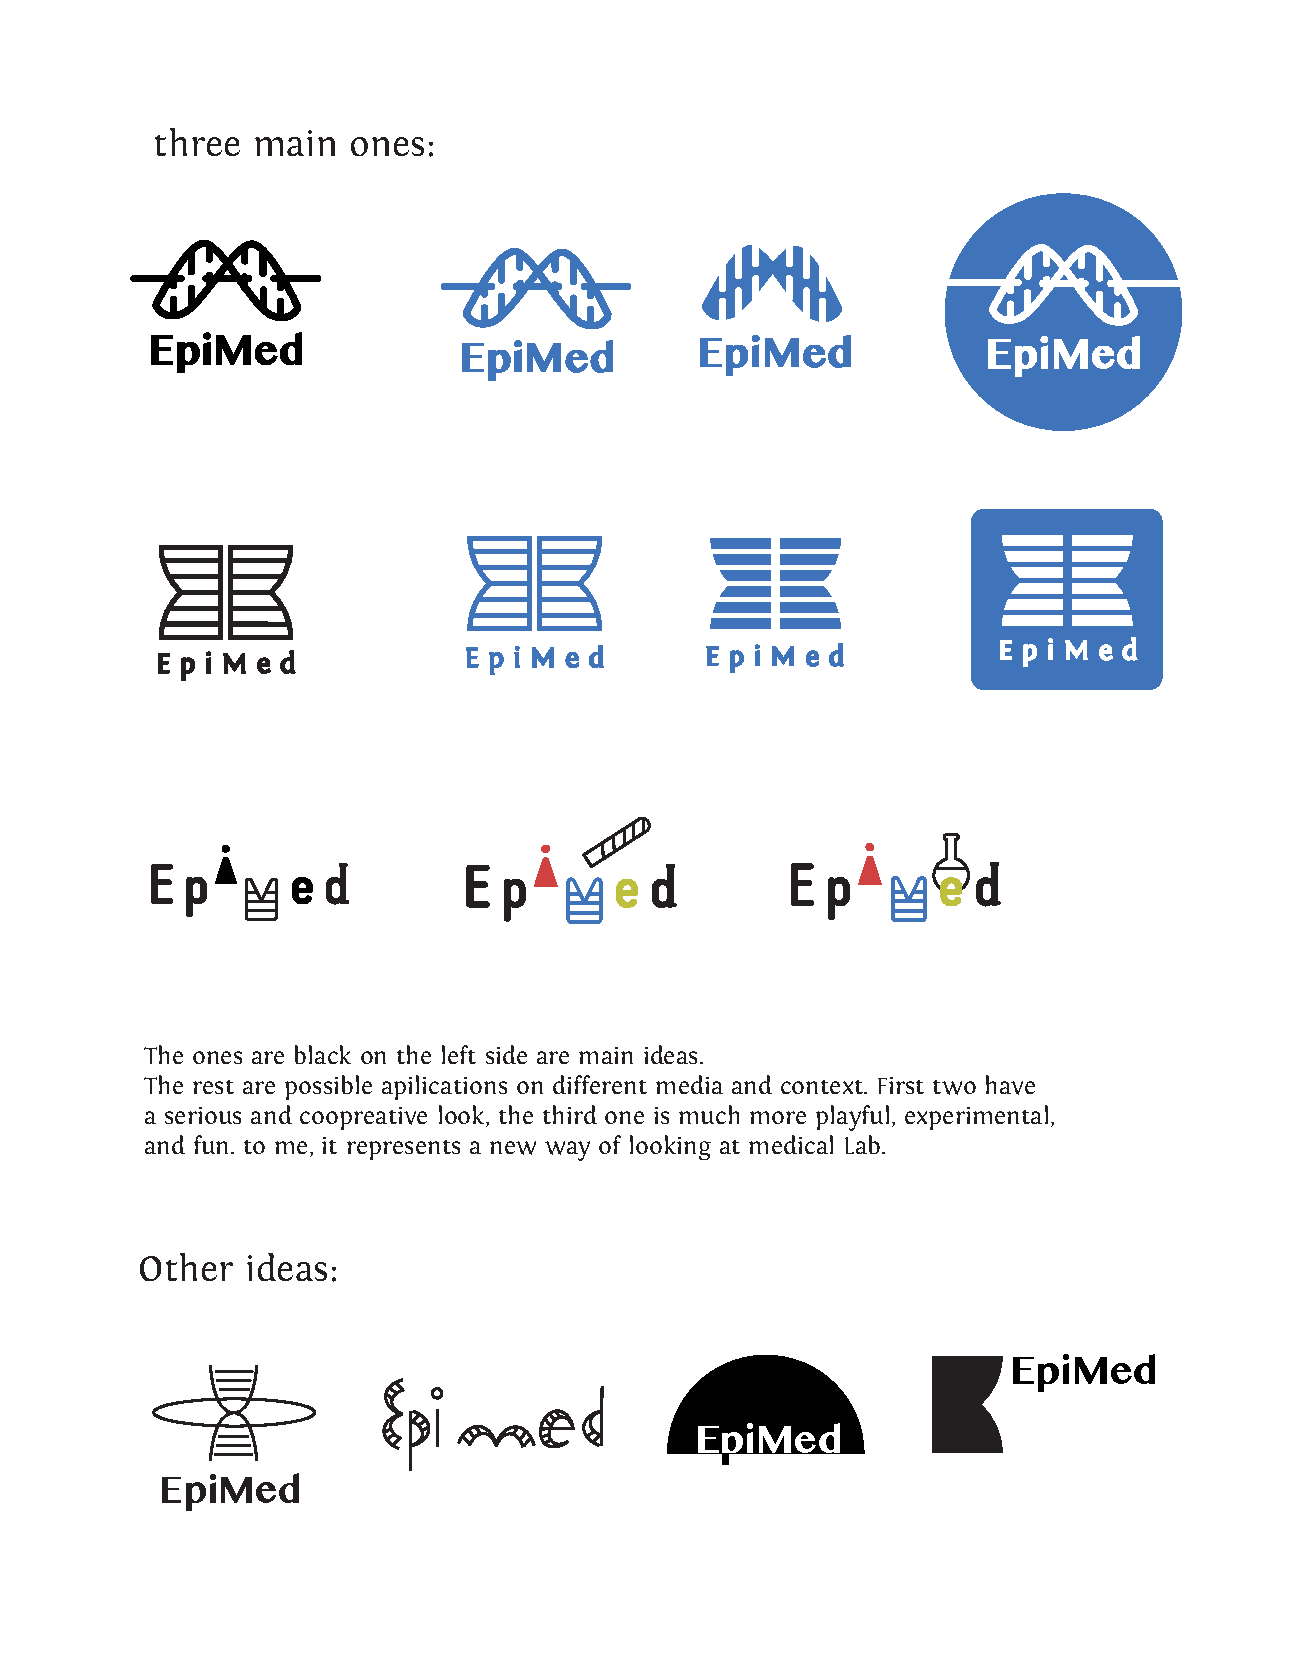
\includegraphics[trim = 150mm 200mm 10mm 32mm, clip, width=0.2\linewidth]{figs/logo_epimed.pdf}
\end{tabular}
\end{center}

%----------------------------------------------------------------------------------------

\end{column} % End of the third column

\end{columns} % End of all the columns in the poster

\end{frame} % End of the enclosing frame

\end{document}
